\documentclass[]{article}
\usepackage{lmodern}
\usepackage{amssymb,amsmath}
\usepackage{ifxetex,ifluatex}
\usepackage{fixltx2e} % provides \textsubscript
\ifnum 0\ifxetex 1\fi\ifluatex 1\fi=0 % if pdftex
  \usepackage[T1]{fontenc}
  \usepackage[utf8]{inputenc}
\else % if luatex or xelatex
  \ifxetex
    \usepackage{mathspec}
  \else
    \usepackage{fontspec}
  \fi
  \defaultfontfeatures{Ligatures=TeX,Scale=MatchLowercase}
\fi
% use upquote if available, for straight quotes in verbatim environments
\IfFileExists{upquote.sty}{\usepackage{upquote}}{}
% use microtype if available
\IfFileExists{microtype.sty}{%
\usepackage{microtype}
\UseMicrotypeSet[protrusion]{basicmath} % disable protrusion for tt fonts
}{}
\usepackage[margin=1in]{geometry}
\usepackage{hyperref}
\hypersetup{unicode=true,
            pdftitle={Effects of Storms in the United States on Population Health and Economy},
            pdfauthor={Dominik Sudwischer},
            pdfborder={0 0 0},
            breaklinks=true}
\urlstyle{same}  % don't use monospace font for urls
\usepackage{color}
\usepackage{fancyvrb}
\newcommand{\VerbBar}{|}
\newcommand{\VERB}{\Verb[commandchars=\\\{\}]}
\DefineVerbatimEnvironment{Highlighting}{Verbatim}{commandchars=\\\{\}}
% Add ',fontsize=\small' for more characters per line
\usepackage{framed}
\definecolor{shadecolor}{RGB}{248,248,248}
\newenvironment{Shaded}{\begin{snugshade}}{\end{snugshade}}
\newcommand{\KeywordTok}[1]{\textcolor[rgb]{0.13,0.29,0.53}{\textbf{{#1}}}}
\newcommand{\DataTypeTok}[1]{\textcolor[rgb]{0.13,0.29,0.53}{{#1}}}
\newcommand{\DecValTok}[1]{\textcolor[rgb]{0.00,0.00,0.81}{{#1}}}
\newcommand{\BaseNTok}[1]{\textcolor[rgb]{0.00,0.00,0.81}{{#1}}}
\newcommand{\FloatTok}[1]{\textcolor[rgb]{0.00,0.00,0.81}{{#1}}}
\newcommand{\ConstantTok}[1]{\textcolor[rgb]{0.00,0.00,0.00}{{#1}}}
\newcommand{\CharTok}[1]{\textcolor[rgb]{0.31,0.60,0.02}{{#1}}}
\newcommand{\SpecialCharTok}[1]{\textcolor[rgb]{0.00,0.00,0.00}{{#1}}}
\newcommand{\StringTok}[1]{\textcolor[rgb]{0.31,0.60,0.02}{{#1}}}
\newcommand{\VerbatimStringTok}[1]{\textcolor[rgb]{0.31,0.60,0.02}{{#1}}}
\newcommand{\SpecialStringTok}[1]{\textcolor[rgb]{0.31,0.60,0.02}{{#1}}}
\newcommand{\ImportTok}[1]{{#1}}
\newcommand{\CommentTok}[1]{\textcolor[rgb]{0.56,0.35,0.01}{\textit{{#1}}}}
\newcommand{\DocumentationTok}[1]{\textcolor[rgb]{0.56,0.35,0.01}{\textbf{\textit{{#1}}}}}
\newcommand{\AnnotationTok}[1]{\textcolor[rgb]{0.56,0.35,0.01}{\textbf{\textit{{#1}}}}}
\newcommand{\CommentVarTok}[1]{\textcolor[rgb]{0.56,0.35,0.01}{\textbf{\textit{{#1}}}}}
\newcommand{\OtherTok}[1]{\textcolor[rgb]{0.56,0.35,0.01}{{#1}}}
\newcommand{\FunctionTok}[1]{\textcolor[rgb]{0.00,0.00,0.00}{{#1}}}
\newcommand{\VariableTok}[1]{\textcolor[rgb]{0.00,0.00,0.00}{{#1}}}
\newcommand{\ControlFlowTok}[1]{\textcolor[rgb]{0.13,0.29,0.53}{\textbf{{#1}}}}
\newcommand{\OperatorTok}[1]{\textcolor[rgb]{0.81,0.36,0.00}{\textbf{{#1}}}}
\newcommand{\BuiltInTok}[1]{{#1}}
\newcommand{\ExtensionTok}[1]{{#1}}
\newcommand{\PreprocessorTok}[1]{\textcolor[rgb]{0.56,0.35,0.01}{\textit{{#1}}}}
\newcommand{\AttributeTok}[1]{\textcolor[rgb]{0.77,0.63,0.00}{{#1}}}
\newcommand{\RegionMarkerTok}[1]{{#1}}
\newcommand{\InformationTok}[1]{\textcolor[rgb]{0.56,0.35,0.01}{\textbf{\textit{{#1}}}}}
\newcommand{\WarningTok}[1]{\textcolor[rgb]{0.56,0.35,0.01}{\textbf{\textit{{#1}}}}}
\newcommand{\AlertTok}[1]{\textcolor[rgb]{0.94,0.16,0.16}{{#1}}}
\newcommand{\ErrorTok}[1]{\textcolor[rgb]{0.64,0.00,0.00}{\textbf{{#1}}}}
\newcommand{\NormalTok}[1]{{#1}}
\usepackage{graphicx,grffile}
\makeatletter
\def\maxwidth{\ifdim\Gin@nat@width>\linewidth\linewidth\else\Gin@nat@width\fi}
\def\maxheight{\ifdim\Gin@nat@height>\textheight\textheight\else\Gin@nat@height\fi}
\makeatother
% Scale images if necessary, so that they will not overflow the page
% margins by default, and it is still possible to overwrite the defaults
% using explicit options in \includegraphics[width, height, ...]{}
\setkeys{Gin}{width=\maxwidth,height=\maxheight,keepaspectratio}
\IfFileExists{parskip.sty}{%
\usepackage{parskip}
}{% else
\setlength{\parindent}{0pt}
\setlength{\parskip}{6pt plus 2pt minus 1pt}
}
\setlength{\emergencystretch}{3em}  % prevent overfull lines
\providecommand{\tightlist}{%
  \setlength{\itemsep}{0pt}\setlength{\parskip}{0pt}}
\setcounter{secnumdepth}{0}
% Redefines (sub)paragraphs to behave more like sections
\ifx\paragraph\undefined\else
\let\oldparagraph\paragraph
\renewcommand{\paragraph}[1]{\oldparagraph{#1}\mbox{}}
\fi
\ifx\subparagraph\undefined\else
\let\oldsubparagraph\subparagraph
\renewcommand{\subparagraph}[1]{\oldsubparagraph{#1}\mbox{}}
\fi

%%% Use protect on footnotes to avoid problems with footnotes in titles
\let\rmarkdownfootnote\footnote%
\def\footnote{\protect\rmarkdownfootnote}

%%% Change title format to be more compact
\usepackage{titling}

% Create subtitle command for use in maketitle
\newcommand{\subtitle}[1]{
  \posttitle{
    \begin{center}\large#1\end{center}
    }
}

\setlength{\droptitle}{-2em}
  \title{Effects of Storms in the United States on Population Health and Economy}
  \pretitle{\vspace{\droptitle}\centering\huge}
  \posttitle{\par}
  \author{Dominik Sudwischer}
  \preauthor{\centering\large\emph}
  \postauthor{\par}
  \predate{\centering\large\emph}
  \postdate{\par}
  \date{29 October 2017}


\begin{document}
\maketitle

\subsection{Synopsis}\label{synopsis}

This analysis examines the U.S. National Oceanic and Atmospheric
Administration's (NOAA) storm database. This database contains records
of storms and related weather events in the United States including
estimations of caused damage. The damage can be categorized in two
groups: population health damage such as injuries or fatalities and
economic damage like destruction of property. Our main goal is to
analyse which type of events were most dangerous to each of the two
categories during the years from 2005 through 2011. Our analysis will
show that the top 3 hazards with direct health impact are tornadoes,
excessive heat and thunderstorms while the destructive force of
hurricanes, flood and - to much less extent - tornadoes and
thunderstorms caused the majority of economic damage.

\subsection{Used Packages}\label{used-packages}

The following packages will be used in this report:

\begin{Shaded}
\begin{Highlighting}[]
\KeywordTok{library}\NormalTok{(lubridate)}
\end{Highlighting}
\end{Shaded}

\begin{verbatim}
## 
## Attaching package: 'lubridate'
\end{verbatim}

\begin{verbatim}
## The following object is masked from 'package:base':
## 
##     date
\end{verbatim}

\begin{Shaded}
\begin{Highlighting}[]
\KeywordTok{library}\NormalTok{(dplyr)}
\end{Highlighting}
\end{Shaded}

\begin{verbatim}
## 
## Attaching package: 'dplyr'
\end{verbatim}

\begin{verbatim}
## The following objects are masked from 'package:lubridate':
## 
##     intersect, setdiff, union
\end{verbatim}

\begin{verbatim}
## The following objects are masked from 'package:stats':
## 
##     filter, lag
\end{verbatim}

\begin{verbatim}
## The following objects are masked from 'package:base':
## 
##     intersect, setdiff, setequal, union
\end{verbatim}

\begin{Shaded}
\begin{Highlighting}[]
\KeywordTok{library}\NormalTok{(ggplot2)}
\end{Highlighting}
\end{Shaded}

\subsection{Data Processing}\label{data-processing}

We start by loading the provided file from the NOAA which contains
records from 1950 to 2011.

\begin{Shaded}
\begin{Highlighting}[]
\NormalTok{df <-}\StringTok{ }\KeywordTok{read.csv}\NormalTok{(}\StringTok{"repdata%2Fdata%2FStormData.csv.bz2"}\NormalTok{)}
\KeywordTok{summary}\NormalTok{(df)}
\end{Highlighting}
\end{Shaded}

\begin{verbatim}
##     STATE__                  BGN_DATE             BGN_TIME     
##  Min.   : 1.0   5/25/2011 0:00:00:  1202   12:00:00 AM: 10163  
##  1st Qu.:19.0   4/27/2011 0:00:00:  1193   06:00:00 PM:  7350  
##  Median :30.0   6/9/2011 0:00:00 :  1030   04:00:00 PM:  7261  
##  Mean   :31.2   5/30/2004 0:00:00:  1016   05:00:00 PM:  6891  
##  3rd Qu.:45.0   4/4/2011 0:00:00 :  1009   12:00:00 PM:  6703  
##  Max.   :95.0   4/2/2006 0:00:00 :   981   03:00:00 PM:  6700  
##                 (Other)          :895866   (Other)    :857229  
##    TIME_ZONE          COUNTY           COUNTYNAME         STATE       
##  CST    :547493   Min.   :  0.0   JEFFERSON :  7840   TX     : 83728  
##  EST    :245558   1st Qu.: 31.0   WASHINGTON:  7603   KS     : 53440  
##  MST    : 68390   Median : 75.0   JACKSON   :  6660   OK     : 46802  
##  PST    : 28302   Mean   :100.6   FRANKLIN  :  6256   MO     : 35648  
##  AST    :  6360   3rd Qu.:131.0   LINCOLN   :  5937   IA     : 31069  
##  HST    :  2563   Max.   :873.0   MADISON   :  5632   NE     : 30271  
##  (Other):  3631                   (Other)   :862369   (Other):621339  
##                EVTYPE         BGN_RANGE           BGN_AZI      
##  HAIL             :288661   Min.   :   0.000          :547332  
##  TSTM WIND        :219940   1st Qu.:   0.000   N      : 86752  
##  THUNDERSTORM WIND: 82563   Median :   0.000   W      : 38446  
##  TORNADO          : 60652   Mean   :   1.484   S      : 37558  
##  FLASH FLOOD      : 54277   3rd Qu.:   1.000   E      : 33178  
##  FLOOD            : 25326   Max.   :3749.000   NW     : 24041  
##  (Other)          :170878                      (Other):134990  
##          BGN_LOCATI                  END_DATE             END_TIME     
##               :287743                    :243411              :238978  
##  COUNTYWIDE   : 19680   4/27/2011 0:00:00:  1214   06:00:00 PM:  9802  
##  Countywide   :   993   5/25/2011 0:00:00:  1196   05:00:00 PM:  8314  
##  SPRINGFIELD  :   843   6/9/2011 0:00:00 :  1021   04:00:00 PM:  8104  
##  SOUTH PORTION:   810   4/4/2011 0:00:00 :  1007   12:00:00 PM:  7483  
##  NORTH PORTION:   784   5/30/2004 0:00:00:   998   11:59:00 PM:  7184  
##  (Other)      :591444   (Other)          :653450   (Other)    :622432  
##    COUNTY_END COUNTYENDN       END_RANGE           END_AZI      
##  Min.   :0    Mode:logical   Min.   :  0.0000          :724837  
##  1st Qu.:0    NA's:902297    1st Qu.:  0.0000   N      : 28082  
##  Median :0                   Median :  0.0000   S      : 22510  
##  Mean   :0                   Mean   :  0.9862   W      : 20119  
##  3rd Qu.:0                   3rd Qu.:  0.0000   E      : 20047  
##  Max.   :0                   Max.   :925.0000   NE     : 14606  
##                                                 (Other): 72096  
##            END_LOCATI         LENGTH              WIDTH         
##                 :499225   Min.   :   0.0000   Min.   :   0.000  
##  COUNTYWIDE     : 19731   1st Qu.:   0.0000   1st Qu.:   0.000  
##  SOUTH PORTION  :   833   Median :   0.0000   Median :   0.000  
##  NORTH PORTION  :   780   Mean   :   0.2301   Mean   :   7.503  
##  CENTRAL PORTION:   617   3rd Qu.:   0.0000   3rd Qu.:   0.000  
##  SPRINGFIELD    :   575   Max.   :2315.0000   Max.   :4400.000  
##  (Other)        :380536                                         
##        F               MAG            FATALITIES          INJURIES        
##  Min.   :0.0      Min.   :    0.0   Min.   :  0.0000   Min.   :   0.0000  
##  1st Qu.:0.0      1st Qu.:    0.0   1st Qu.:  0.0000   1st Qu.:   0.0000  
##  Median :1.0      Median :   50.0   Median :  0.0000   Median :   0.0000  
##  Mean   :0.9      Mean   :   46.9   Mean   :  0.0168   Mean   :   0.1557  
##  3rd Qu.:1.0      3rd Qu.:   75.0   3rd Qu.:  0.0000   3rd Qu.:   0.0000  
##  Max.   :5.0      Max.   :22000.0   Max.   :583.0000   Max.   :1700.0000  
##  NA's   :843563                                                           
##     PROPDMG          PROPDMGEXP        CROPDMG          CROPDMGEXP    
##  Min.   :   0.00          :465934   Min.   :  0.000          :618413  
##  1st Qu.:   0.00   K      :424665   1st Qu.:  0.000   K      :281832  
##  Median :   0.00   M      : 11330   Median :  0.000   M      :  1994  
##  Mean   :  12.06   0      :   216   Mean   :  1.527   k      :    21  
##  3rd Qu.:   0.50   B      :    40   3rd Qu.:  0.000   0      :    19  
##  Max.   :5000.00   5      :    28   Max.   :990.000   B      :     9  
##                    (Other):    84                     (Other):     9  
##       WFO                                       STATEOFFIC    
##         :142069                                      :248769  
##  OUN    : 17393   TEXAS, North                       : 12193  
##  JAN    : 13889   ARKANSAS, Central and North Central: 11738  
##  LWX    : 13174   IOWA, Central                      : 11345  
##  PHI    : 12551   KANSAS, Southwest                  : 11212  
##  TSA    : 12483   GEORGIA, North and Central         : 11120  
##  (Other):690738   (Other)                            :595920  
##                                                                                                                                                                                                     ZONENAMES     
##                                                                                                                                                                                                          :594029  
##                                                                                                                                                                                                          :205988  
##  GREATER RENO / CARSON CITY / M - GREATER RENO / CARSON CITY / M                                                                                                                                         :   639  
##  GREATER LAKE TAHOE AREA - GREATER LAKE TAHOE AREA                                                                                                                                                       :   592  
##  JEFFERSON - JEFFERSON                                                                                                                                                                                   :   303  
##  MADISON - MADISON                                                                                                                                                                                       :   302  
##  (Other)                                                                                                                                                                                                 :100444  
##     LATITUDE      LONGITUDE        LATITUDE_E     LONGITUDE_    
##  Min.   :   0   Min.   :-14451   Min.   :   0   Min.   :-14455  
##  1st Qu.:2802   1st Qu.:  7247   1st Qu.:   0   1st Qu.:     0  
##  Median :3540   Median :  8707   Median :   0   Median :     0  
##  Mean   :2875   Mean   :  6940   Mean   :1452   Mean   :  3509  
##  3rd Qu.:4019   3rd Qu.:  9605   3rd Qu.:3549   3rd Qu.:  8735  
##  Max.   :9706   Max.   : 17124   Max.   :9706   Max.   :106220  
##  NA's   :47                      NA's   :40                     
##                                            REMARKS           REFNUM      
##                                                :287433   Min.   :     1  
##                                                : 24013   1st Qu.:225575  
##  Trees down.\n                                 :  1110   Median :451149  
##  Several trees were blown down.\n              :   568   Mean   :451149  
##  Trees were downed.\n                          :   446   3rd Qu.:676723  
##  Large trees and power lines were blown down.\n:   432   Max.   :902297  
##  (Other)                                       :588295
\end{verbatim}

The data contains more than 900000 observations with 37 variables in
total. The event type is stored as a factor in the ``EVTYPE'' column and
has 985 levels, some of which indicate summaries and some of which still
have to be combined. We will investigate which events are the most
hazardous in terms of health damage or property damage.

The data is a bit unclean, so we will need to do some work before can we
can analyse the data. We start with transforming letters to lower case
in columns describing the events and columns specifying damage
multipliers (the ``\ldots{}exp'' columns with factors like ``M'', ``k''
and so on).

\begin{Shaded}
\begin{Highlighting}[]
\NormalTok{df[, }\KeywordTok{c}\NormalTok{(}\StringTok{"CROPDMGEXP"}\NormalTok{, }\StringTok{"PROPDMGEXP"}\NormalTok{, }\StringTok{"EVTYPE"}\NormalTok{)] <-}
\StringTok{  }\KeywordTok{data.frame}\NormalTok{(}\KeywordTok{sapply}\NormalTok{(df[, }\KeywordTok{c}\NormalTok{(}\StringTok{"CROPDMGEXP"}\NormalTok{, }\StringTok{"PROPDMGEXP"}\NormalTok{, }\StringTok{"EVTYPE"}\NormalTok{)], tolower))}
\KeywordTok{unique}\NormalTok{(df$CROPDMGEXP)}
\end{Highlighting}
\end{Shaded}

\begin{verbatim}
## [1]   m k b ? 0 2
## Levels:  ? 0 2 b k m
\end{verbatim}

\begin{Shaded}
\begin{Highlighting}[]
\KeywordTok{unique}\NormalTok{(df$PROPDMGEXP)}
\end{Highlighting}
\end{Shaded}

\begin{verbatim}
##  [1] k m   b + 0 5 6 ? 4 2 3 h 7 - 1 8
## Levels:  - ? + 0 1 2 3 4 5 6 7 8 b h k m
\end{verbatim}

The data ``exp'' columns indicate the power of 10 that should be
multiplied with the number in the actual damage column. The values
``?'', ``+'' and ``-'' are not usable because they do not clearly state
what they stand for, so we will remove those lines. A blank entry
corresponds to the factor 1 (or the exponent 0). Other than that, ``b''
(billion) is 10\^{}9, ``m'' (mega) is 10\^{}6, ``k'' (kilo) is 10\^{}3
and ``h'' (hecto) is 10\^{}2. We will add a new column,
``TOTALECONDMG'', by multiplying crop and property damage by their
respective factors and adding them.

\begin{Shaded}
\begin{Highlighting}[]
\NormalTok{selection <-}\StringTok{ }\NormalTok{!((df$CROPDMGEXP %in%}\StringTok{ }\KeywordTok{c}\NormalTok{(}\StringTok{"+"}\NormalTok{, }\StringTok{"-"}\NormalTok{, }\StringTok{"?"}\NormalTok{)) |}
\StringTok{                 }\NormalTok{(df$PROPDMGEXP %in%}\StringTok{ }\KeywordTok{c}\NormalTok{(}\StringTok{"+"}\NormalTok{, }\StringTok{"-"}\NormalTok{, }\StringTok{"?"}\NormalTok{)))}
\NormalTok{df <-}\StringTok{ }\NormalTok{df[selection, ]}
\NormalTok{df$PROPDMGFACTOR <-}\StringTok{ }\DecValTok{1}
\NormalTok{df$PROPDMGFACTOR[df$PROPDMGEXP ==}\StringTok{ "h"}\NormalTok{] <-}\StringTok{ }\DecValTok{100}
\NormalTok{df$PROPDMGFACTOR[df$PROPDMGEXP ==}\StringTok{ "k"}\NormalTok{] <-}\StringTok{ }\DecValTok{1000}
\NormalTok{df$PROPDMGFACTOR[df$PROPDMGEXP ==}\StringTok{ "m"}\NormalTok{] <-}\StringTok{ }\DecValTok{1000000}
\NormalTok{df$PROPDMGFACTOR[df$PROPDMGEXP ==}\StringTok{ "b"}\NormalTok{] <-}\StringTok{ }\DecValTok{1000000000}
\NormalTok{selection <-}\StringTok{ }\NormalTok{!}\KeywordTok{is.na}\NormalTok{(}\KeywordTok{as.numeric}\NormalTok{(df$PROPDMGEXP))}
\NormalTok{df$CROPDMGFACTOR[selection] <-}\StringTok{ }\DecValTok{10}\NormalTok{^}\KeywordTok{as.numeric}\NormalTok{(df$CROPDMGEXP[selection])}
\NormalTok{df$CROPDMGFACTOR <-}\StringTok{ }\DecValTok{1}
\NormalTok{df$CROPDMGFACTOR[df$CROPDMGEXP ==}\StringTok{ "h"}\NormalTok{] <-}\StringTok{ }\DecValTok{100}
\NormalTok{df$CROPDMGFACTOR[df$CROPDMGEXP ==}\StringTok{ "k"}\NormalTok{] <-}\StringTok{ }\DecValTok{1000}
\NormalTok{df$CROPDMGFACTOR[df$CROPDMGEXP ==}\StringTok{ "m"}\NormalTok{] <-}\StringTok{ }\DecValTok{1000000}
\NormalTok{df$CROPDMGFACTOR[df$CROPDMGEXP ==}\StringTok{ "b"}\NormalTok{] <-}\StringTok{ }\DecValTok{1000000000}
\NormalTok{selection <-}\StringTok{ }\NormalTok{!}\KeywordTok{is.na}\NormalTok{(}\KeywordTok{as.numeric}\NormalTok{(df$CROPDMGEXP))}
\NormalTok{df$CROPDMGFACTOR[selection] <-}\StringTok{ }\DecValTok{10}\NormalTok{^}\KeywordTok{as.numeric}\NormalTok{(df$CROPDMGEXP[selection])}
\NormalTok{df$TOTALECONDMG <-}\StringTok{ }\KeywordTok{as.numeric}\NormalTok{(df$CROPDMG) *}
\StringTok{  }\KeywordTok{as.numeric}\NormalTok{(df$PROPDMGFACTOR) +}
\StringTok{  }\KeywordTok{as.numeric}\NormalTok{(df$PROPDMG) *}
\StringTok{  }\KeywordTok{as.numeric}\NormalTok{(df$PROPDMGFACTOR)}
\end{Highlighting}
\end{Shaded}

Now that we have useful data for economic damage, we will clean the
event descriptions. The data uses different words for similar weather
events such as ``very dry'' and ``drought''. We will consolidate the
data a bit. However, since there are 985 different factor levels, a very
sophisticated method for consolidation is difficult to develop and
beyond the scope of this report. Instead we will use a simpler method.

\begin{Shaded}
\begin{Highlighting}[]
\NormalTok{consolidate <-}\StringTok{ }\NormalTok{function(event)}
\NormalTok{\{}
  \NormalTok{if(}\KeywordTok{grepl}\NormalTok{(}\StringTok{"hurricane|typhoon|cyclone"}\NormalTok{, event))}
  \NormalTok{\{ }\StringTok{"hurricane"} \NormalTok{\}}
  \NormalTok{else if(}\KeywordTok{grepl}\NormalTok{(}\StringTok{"tornado"}\NormalTok{, event))}
    \NormalTok{\{ }\StringTok{"tornado"} \NormalTok{\}}
  \NormalTok{else if(}\KeywordTok{grepl}\NormalTok{(}\StringTok{"drought|dry|hot|heat|warm|high temp|warmth"}\NormalTok{, event))}
    \NormalTok{\{ }\StringTok{"heatwave"} \NormalTok{\}}
  \NormalTok{else if(}\KeywordTok{grepl}\NormalTok{(}\StringTok{"blizzard|hail|snow|glaze"}\NormalTok{, event))}
    \NormalTok{\{ }\StringTok{"blizzard"} \NormalTok{\}}
  \NormalTok{else if(}\KeywordTok{grepl}\NormalTok{(}\StringTok{"tstm|thunderstorm|wind"}\NormalTok{, event))}
    \NormalTok{\{ }\StringTok{"thunderstorm or heavy wind"} \NormalTok{\}}
  \NormalTok{else if(}\KeywordTok{grepl}\NormalTok{(}\StringTok{"rain|wet"}\NormalTok{, event))}
    \NormalTok{\{ }\StringTok{"rainfall"} \NormalTok{\}}
  \NormalTok{else if(}\KeywordTok{grepl}\NormalTok{(}\StringTok{"ice|icy|cold|low temp|freez"}\NormalTok{, event))}
  \NormalTok{\{ }\StringTok{"low temperature"} \NormalTok{\}}
  \NormalTok{else if(}\KeywordTok{grepl}\NormalTok{(}\StringTok{"flood|surge"}\NormalTok{, event))}
    \NormalTok{\{ }\StringTok{"flood"} \NormalTok{\}}
  \NormalTok{else \{ event \}}
\NormalTok{\}}
\end{Highlighting}
\end{Shaded}

We can now modify the event column using this function.

\begin{Shaded}
\begin{Highlighting}[]
\NormalTok{df$EVTYPE <-}\StringTok{ }\KeywordTok{as.factor}\NormalTok{(}\KeywordTok{sapply}\NormalTok{(}\KeywordTok{as.character}\NormalTok{(df$EVTYPE), consolidate))}
\end{Highlighting}
\end{Shaded}

We will focus our research to work with recent calamities, considering
only data from 2005 up to 2011. For this reason, we will begin with a
suitable date conversion of the BGN\_DATE column.

\begin{Shaded}
\begin{Highlighting}[]
\NormalTok{df$YEAR <-}\StringTok{ }\KeywordTok{year}\NormalTok{(}\KeywordTok{as.Date.character}\NormalTok{(df$BGN_DATE, }\DataTypeTok{format =} \StringTok{"%m/%d/%Y"}\NormalTok{))}
\end{Highlighting}
\end{Shaded}

\subsubsection{Selecting a Suitable Subset of the
Data}\label{selecting-a-suitable-subset-of-the-data}

We will create a copy of our original data frame that only contains a
subset of the records, in particular it will comprise all records from
2005 through 2011.

\begin{Shaded}
\begin{Highlighting}[]
\NormalTok{records <-}\StringTok{ }\NormalTok{df[df$YEAR >=}\StringTok{ }\DecValTok{2005}\NormalTok{, ]}
\end{Highlighting}
\end{Shaded}

As we can see, we selected a bit more than a third of the original data
set. The density of reports and the recent years has inceased
drastically, so it is natural that a small subset of the most recent
observed years contains a large proportion of the records.

We will need to observe economic and health damage seperately, so we
will split our data accordingly. \#\#\# Splitting the Data for Further
Analysis

\begin{Shaded}
\begin{Highlighting}[]
\NormalTok{health_df <-}\StringTok{ }\NormalTok{records[, }\KeywordTok{c}\NormalTok{(}\StringTok{"INJURIES"}\NormalTok{, }\StringTok{"FATALITIES"}\NormalTok{, }\StringTok{"EVTYPE"}\NormalTok{)]}
\NormalTok{econ_df <-}\StringTok{ }\NormalTok{records[, }\KeywordTok{c}\NormalTok{(}\StringTok{"TOTALECONDMG"}\NormalTok{, }\StringTok{"EVTYPE"}\NormalTok{)]}
\end{Highlighting}
\end{Shaded}

Next, we check our subset of the data for missing values.

\begin{Shaded}
\begin{Highlighting}[]
\KeywordTok{sum}\NormalTok{(}\KeywordTok{matrix}\NormalTok{(}\DataTypeTok{data =} \KeywordTok{is.na}\NormalTok{(health_df), }\DataTypeTok{ncol =} \DecValTok{1}\NormalTok{))}
\end{Highlighting}
\end{Shaded}

\begin{verbatim}
## [1] 0
\end{verbatim}

\begin{Shaded}
\begin{Highlighting}[]
\KeywordTok{sum}\NormalTok{(}\KeywordTok{matrix}\NormalTok{(}\DataTypeTok{data =} \KeywordTok{is.na}\NormalTok{(econ_df), }\DataTypeTok{ncol =} \DecValTok{1}\NormalTok{))}
\end{Highlighting}
\end{Shaded}

\begin{verbatim}
## [1] 0
\end{verbatim}

Neither of our data frames have NA values, so we can continue analysing
the data. We will begin with the health data by grouping by event and
summing up injuries and fatalities. We will also introduce a variable
called ``DAMAGE'' which is the weighted sum of injuries (with factor 1)
and fatalities (with factor 4). Additionally, we will sort the data by
this new column in descending order.

\begin{Shaded}
\begin{Highlighting}[]
\NormalTok{health_df_agg <-}\StringTok{ }\NormalTok{health_df[, }\KeywordTok{c}\NormalTok{(}\StringTok{"INJURIES"}\NormalTok{, }\StringTok{"FATALITIES"}\NormalTok{)] %>%}
\StringTok{  }\KeywordTok{group_by}\NormalTok{(health_df$EVTYPE) %>%}\StringTok{ }\KeywordTok{summarise_all}\NormalTok{(}\KeywordTok{funs}\NormalTok{(sum))}
\NormalTok{health_df_agg$DAMAGE =}\StringTok{ }\NormalTok{health_df_agg$INJURIES +}\StringTok{ }\DecValTok{4} \NormalTok{*}\StringTok{ }\NormalTok{health_df_agg$FATALITIES}
\NormalTok{health_df_agg <-}\StringTok{ }\NormalTok{health_df_agg[}\KeywordTok{order}\NormalTok{(-health_df_agg$DAMAGE, -health_df_agg$FATALITIES), ]}
\KeywordTok{colnames}\NormalTok{(health_df_agg)[}\DecValTok{1}\NormalTok{] =}\StringTok{ "EVTYPE"}
\end{Highlighting}
\end{Shaded}

We will do the same for recorded cases of economic damage.

\begin{Shaded}
\begin{Highlighting}[]
\NormalTok{econ_df_agg <-}\StringTok{ }\NormalTok{econ_df %>%}\StringTok{ }\KeywordTok{group_by}\NormalTok{(econ_df$EVTYPE) %>%}
\StringTok{  }\KeywordTok{summarise}\NormalTok{(}\DataTypeTok{TOTALECONDMG =} \KeywordTok{sum}\NormalTok{(TOTALECONDMG))}
\NormalTok{econ_df_agg <-}\StringTok{ }\NormalTok{econ_df_agg[}\KeywordTok{order}\NormalTok{(-econ_df_agg$TOTALECONDMG), ]}
\KeywordTok{colnames}\NormalTok{(econ_df_agg)[}\DecValTok{1}\NormalTok{] =}\StringTok{ "EVTYPE"}
\end{Highlighting}
\end{Shaded}

\subsection{Results}\label{results}

In this section, we will use the multiplot function. The code and the
source can be found in the appendix.

The preparations performed above allow us to generate insights from the
data. We will begin with a bar plot of the 6 top hazards for health and
for the economy.

\begin{Shaded}
\begin{Highlighting}[]
\NormalTok{g <-}\StringTok{ }\KeywordTok{ggplot}\NormalTok{(}\DataTypeTok{data=}\KeywordTok{head}\NormalTok{(health_df_agg), }\KeywordTok{aes}\NormalTok{(}\KeywordTok{reorder}\NormalTok{(EVTYPE, -DAMAGE), DAMAGE)) +}
\StringTok{  }\KeywordTok{geom_bar}\NormalTok{(}\DataTypeTok{stat =} \StringTok{"identity"}\NormalTok{, }\DataTypeTok{fill=}\StringTok{"#FF9999"}\NormalTok{, }\DataTypeTok{color =} \StringTok{"black"}\NormalTok{) +}\StringTok{ }
\StringTok{  }\KeywordTok{labs}\NormalTok{(}\DataTypeTok{x =} \StringTok{"Weather Event"}\NormalTok{, }\DataTypeTok{y =} \StringTok{"Weighted Population Damage"}\NormalTok{,}
       \DataTypeTok{caption =} \StringTok{"Weighted Population Damage of Various Weather}\CharTok{\textbackslash{}n}\StringTok{Events from 2005 to 2011"}\NormalTok{) +}\StringTok{ }
\StringTok{  }\CommentTok{#ggtitle("Weighted Population Damage of Various Weather Events from 2005 to 2011") + }
\StringTok{  }\KeywordTok{theme}\NormalTok{(}\DataTypeTok{axis.text.x =} \KeywordTok{element_text}\NormalTok{(}\DataTypeTok{angle =} \DecValTok{45}\NormalTok{, }\DataTypeTok{hjust =} \DecValTok{1}\NormalTok{))}
\NormalTok{h <-}\StringTok{ }\KeywordTok{ggplot}\NormalTok{(}\DataTypeTok{data=}\KeywordTok{head}\NormalTok{(econ_df_agg), }\KeywordTok{aes}\NormalTok{(}\KeywordTok{reorder}\NormalTok{(EVTYPE, -TOTALECONDMG), TOTALECONDMG)) +}
\StringTok{  }\KeywordTok{geom_bar}\NormalTok{(}\DataTypeTok{stat =} \StringTok{"identity"}\NormalTok{, }\DataTypeTok{fill=}\StringTok{"#FF9999"}\NormalTok{, }\DataTypeTok{color =} \StringTok{"black"}\NormalTok{) +}\StringTok{ }
\StringTok{  }\KeywordTok{labs}\NormalTok{(}\DataTypeTok{x =} \StringTok{"Weather Event"}\NormalTok{, }\DataTypeTok{y =} \StringTok{"Economic Damage"}\NormalTok{,}
       \DataTypeTok{caption =} \StringTok{"Economic Damage of Various Weather}\CharTok{\textbackslash{}n}\StringTok{Events from 2005 to 2011 in USD"}\NormalTok{) +}\StringTok{ }
\StringTok{  }\CommentTok{#ggtitle("Economic Damage of Various Weather Events from 2005 to 2011") + }
\StringTok{  }\KeywordTok{theme}\NormalTok{(}\DataTypeTok{axis.text.x =} \KeywordTok{element_text}\NormalTok{(}\DataTypeTok{angle =} \DecValTok{45}\NormalTok{, }\DataTypeTok{hjust =} \DecValTok{1}\NormalTok{))}
\KeywordTok{multiplot}\NormalTok{(g, h, }\DataTypeTok{cols =} \DecValTok{2}\NormalTok{)}
\end{Highlighting}
\end{Shaded}

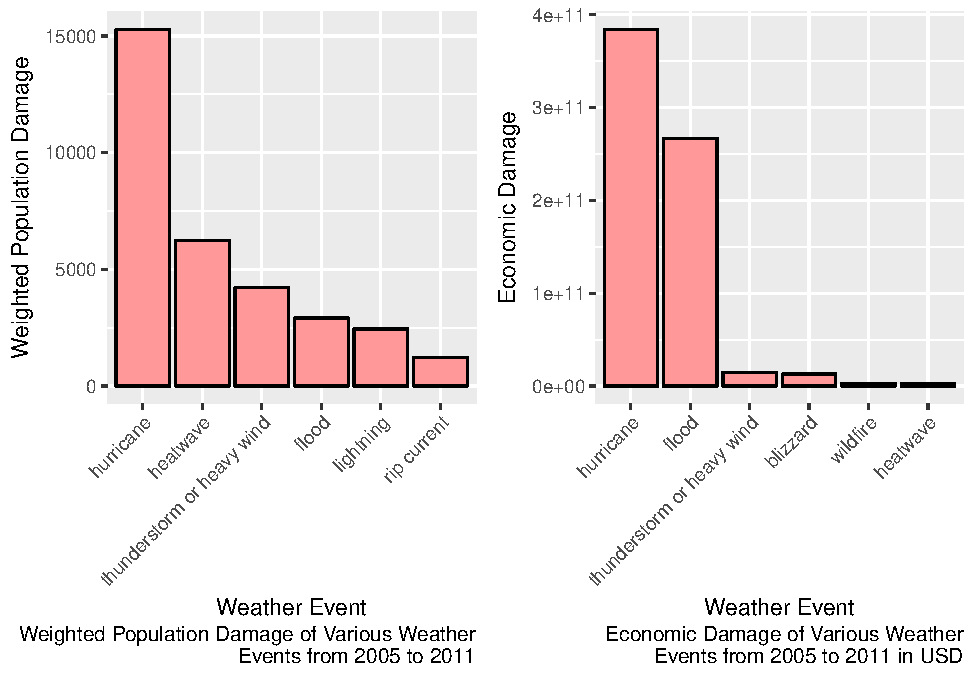
\includegraphics{StormData_files/figure-latex/damage_plots-1.pdf}

We can easily see that hurricanes have a tremendous impact on health
according to our weighted damage, followed by excessive heat and
thunderstorms with much lower numbers. In particular, the numbers of
injuries and fatalities due to the 3 most dangerous hazards is as
follows:

\begin{Shaded}
\begin{Highlighting}[]
\NormalTok{health_df_agg[health_df_agg$EVTYPE %in%}\StringTok{ }\KeywordTok{c}\NormalTok{(}\StringTok{"tornado"}\NormalTok{, }\StringTok{"heatwave"}\NormalTok{,}
                                          \StringTok{"thunderstorm or heavy wind"}\NormalTok{), ]}
\end{Highlighting}
\end{Shaded}

\begin{verbatim}
## # A tibble: 3 x 4
##                       EVTYPE INJURIES FATALITIES DAMAGE
##                       <fctr>    <dbl>      <dbl>  <dbl>
## 1                    tornado    11137        968  15009
## 2                   heatwave     3397        711   6241
## 3 thunderstorm or heavy wind     2283        486   4227
\end{verbatim}

As for economic damage, hurricanes cause enormous damage as well. Second
to them are only flood and far, far behind tornadoes and thunderstorms.
The numbers can be seen below:

\begin{Shaded}
\begin{Highlighting}[]
\NormalTok{econ_df_agg[econ_df_agg$EVTYPE %in%}\StringTok{ }\KeywordTok{c}\NormalTok{(}\StringTok{"hurricane"}\NormalTok{, }\StringTok{"flood"}\NormalTok{, }\StringTok{"tornado"}\NormalTok{, }\StringTok{"thunderstorm or heavy wind"}\NormalTok{), ]}
\end{Highlighting}
\end{Shaded}

\begin{verbatim}
## # A tibble: 4 x 2
##                       EVTYPE TOTALECONDMG
##                       <fctr>        <dbl>
## 1                  hurricane 355336906330
## 2                      flood 266995036151
## 3                    tornado  29057210037
## 4 thunderstorm or heavy wind  15045093540
\end{verbatim}

Finally, we will have a glance at the trend for fatalities by tornadoes
since the beginning of the observations.

\begin{Shaded}
\begin{Highlighting}[]
\NormalTok{tornado_data <-}\StringTok{ }\NormalTok{df[df$EVTYPE ==}\StringTok{ "tornado"}\NormalTok{, }\KeywordTok{c}\NormalTok{(}\StringTok{"FATALITIES"}\NormalTok{, }\StringTok{"YEAR"}\NormalTok{)]}
\NormalTok{tornado_data <-}\StringTok{ }\NormalTok{tornado_data %>%}\StringTok{ }\KeywordTok{group_by}\NormalTok{(tornado_data$YEAR) %>%}
\StringTok{  }\KeywordTok{summarise}\NormalTok{(}\DataTypeTok{SUM_FATALITIES =} \KeywordTok{sum}\NormalTok{(FATALITIES))}
\KeywordTok{colnames}\NormalTok{(tornado_data)[}\DecValTok{1}\NormalTok{] =}\StringTok{ "YEAR"}
\NormalTok{g <-}\StringTok{ }\KeywordTok{ggplot}\NormalTok{(}\DataTypeTok{data=}\NormalTok{tornado_data, }\KeywordTok{aes}\NormalTok{(YEAR)) +}
\StringTok{  }\KeywordTok{geom_line}\NormalTok{(}\KeywordTok{aes}\NormalTok{(}\DataTypeTok{y =} \NormalTok{tornado_data$SUM_FATALITIES)) +}\StringTok{ }
\StringTok{  }\KeywordTok{scale_x_continuous}\NormalTok{(}\DataTypeTok{breaks =} \KeywordTok{seq}\NormalTok{(}\DecValTok{1950}\NormalTok{, }\DecValTok{2011}\NormalTok{, }\DecValTok{5}\NormalTok{), }\StringTok{"Year"}\NormalTok{) +}
\StringTok{  }\KeywordTok{labs}\NormalTok{(}\DataTypeTok{x =} \StringTok{"Year"}\NormalTok{, }\DataTypeTok{y =} \StringTok{"Injuries"}\NormalTok{,}
       \DataTypeTok{caption =} \StringTok{"Fatalities by Tornadoes per Year"}\NormalTok{) +}\StringTok{ }
\StringTok{  }\KeywordTok{theme}\NormalTok{(}\DataTypeTok{axis.text.x =} \KeywordTok{element_text}\NormalTok{(}\DataTypeTok{angle =} \DecValTok{45}\NormalTok{, }\DataTypeTok{hjust =} \DecValTok{1}\NormalTok{))}
\NormalTok{g}
\end{Highlighting}
\end{Shaded}

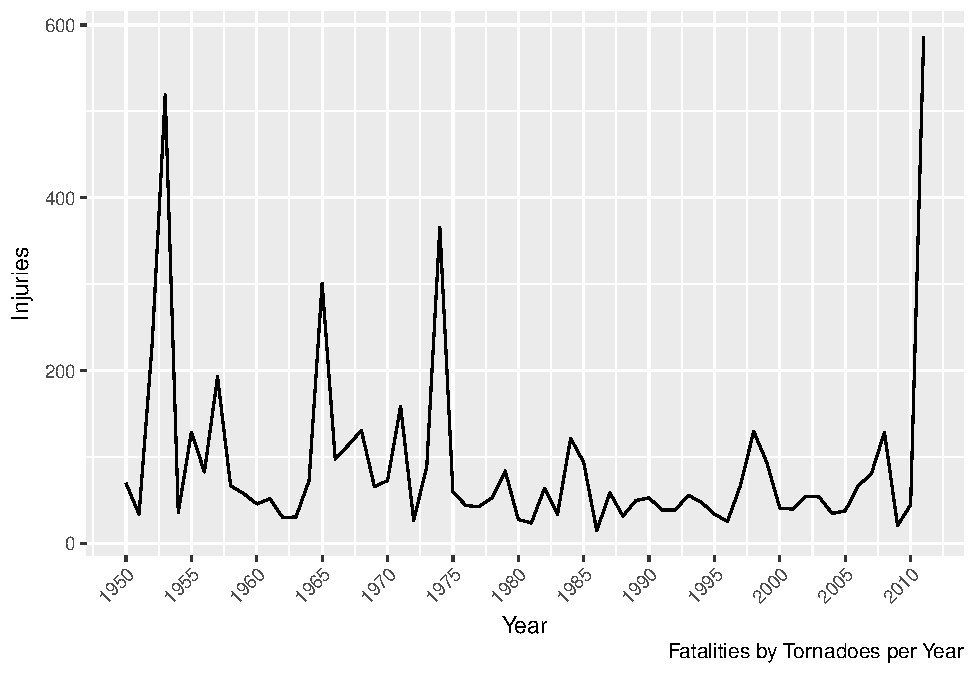
\includegraphics{StormData_files/figure-latex/prepare_data_for_tornado_graph-1.pdf}

As we can see, there are some spikes in the data corresponding to
extraordinarily threatening tornadoes.

We conclude our analysis with the remark that the most dangerous hazards
for population health are indeed tornadoes, excessive heat and
thunderstorms. The most economic damage is caused by hurricanes and
flood.

\subsection{Appendix}\label{appendix}

This is the definition of the multiplot function.
\href{http://www.cookbook-r.com/Graphs/Multiple_graphs_on_one_page_(ggplot2)}{Source}:

\begin{Shaded}
\begin{Highlighting}[]
\CommentTok{# Multiple plot function}
\CommentTok{#}
\CommentTok{# ggplot objects can be passed in ..., or to plotlist (as a list of ggplot objects)}
\CommentTok{# - cols:   Number of columns in layout}
\CommentTok{# - layout: A matrix specifying the layout. If present, 'cols' is ignored.}
\CommentTok{#}
\CommentTok{# If the layout is something like matrix(c(1,2,3,3), nrow=2, byrow=TRUE),}
\CommentTok{# then plot 1 will go in the upper left, 2 will go in the upper right, and}
\CommentTok{# 3 will go all the way across the bottom.}
\CommentTok{#}
\NormalTok{multiplot <-}\StringTok{ }\NormalTok{function(..., }\DataTypeTok{plotlist=}\OtherTok{NULL}\NormalTok{, file, }\DataTypeTok{cols=}\DecValTok{1}\NormalTok{, }\DataTypeTok{layout=}\OtherTok{NULL}\NormalTok{) \{}
  \KeywordTok{library}\NormalTok{(grid)}

  \CommentTok{# Make a list from the ... arguments and plotlist}
  \NormalTok{plots <-}\StringTok{ }\KeywordTok{c}\NormalTok{(}\KeywordTok{list}\NormalTok{(...), plotlist)}

  \NormalTok{numPlots =}\StringTok{ }\KeywordTok{length}\NormalTok{(plots)}

  \CommentTok{# If layout is NULL, then use 'cols' to determine layout}
  \NormalTok{if (}\KeywordTok{is.null}\NormalTok{(layout)) \{}
    \CommentTok{# Make the panel}
    \CommentTok{# ncol: Number of columns of plots}
    \CommentTok{# nrow: Number of rows needed, calculated from # of cols}
    \NormalTok{layout <-}\StringTok{ }\KeywordTok{matrix}\NormalTok{(}\KeywordTok{seq}\NormalTok{(}\DecValTok{1}\NormalTok{, cols *}\StringTok{ }\KeywordTok{ceiling}\NormalTok{(numPlots/cols)),}
                    \DataTypeTok{ncol =} \NormalTok{cols, }\DataTypeTok{nrow =} \KeywordTok{ceiling}\NormalTok{(numPlots/cols))}
  \NormalTok{\}}

 \NormalTok{if (numPlots==}\DecValTok{1}\NormalTok{) \{}
    \KeywordTok{print}\NormalTok{(plots[[}\DecValTok{1}\NormalTok{]])}

  \NormalTok{\} else \{}
    \CommentTok{# Set up the page}
    \KeywordTok{grid.newpage}\NormalTok{()}
    \KeywordTok{pushViewport}\NormalTok{(}\KeywordTok{viewport}\NormalTok{(}\DataTypeTok{layout =} \KeywordTok{grid.layout}\NormalTok{(}\KeywordTok{nrow}\NormalTok{(layout), }\KeywordTok{ncol}\NormalTok{(layout))))}

    \CommentTok{# Make each plot, in the correct location}
    \NormalTok{for (i in }\DecValTok{1}\NormalTok{:numPlots) \{}
      \CommentTok{# Get the i,j matrix positions of the regions that contain this subplot}
      \NormalTok{matchidx <-}\StringTok{ }\KeywordTok{as.data.frame}\NormalTok{(}\KeywordTok{which}\NormalTok{(layout ==}\StringTok{ }\NormalTok{i, }\DataTypeTok{arr.ind =} \OtherTok{TRUE}\NormalTok{))}

      \KeywordTok{print}\NormalTok{(plots[[i]], }\DataTypeTok{vp =} \KeywordTok{viewport}\NormalTok{(}\DataTypeTok{layout.pos.row =} \NormalTok{matchidx$row,}
                                      \DataTypeTok{layout.pos.col =} \NormalTok{matchidx$col))}
    \NormalTok{\}}
  \NormalTok{\}}
\NormalTok{\}}
\end{Highlighting}
\end{Shaded}


\end{document}
